\TransitionFrame{confronto di tecniche per la cinematica inversa}

\begin{frame}{Framework}

% loghi
\begin{columns}
\begin{column}{0.5\textwidth}
\begin{center} TRAC-IK\end{center}
\begin{center}
    
\includegraphics[width=0.2\textwidth]{slide/img_cinematica_inversa/trac-ik.png}
\end{center}
\end{column}
\begin{column}{0.5\textwidth}
\begin{center} SCIPY\end{center}
\begin{center}
    
\includegraphics[width=0.4\textwidth]{slide/img_cinematica_inversa/scipy.png}
\end{center}
\end{column}
\end{columns}

% descrizione
\begin{columns}
\begin{column}{0.5\textwidth}
\begin{itemize}
    \item<1-> ottimizzazione applicata alla cinematica inversa
    \item<4-> package del framework ROS
    \item<6-> Newton + SLSQP
\end{itemize}
\end{column}
\begin{column}{0.5\textwidth}
\begin{itemize}
    \item<2-> ottimizzazione ``general purpose"
    \begin{itemize}
        \item<3-> flessibile
    \end{itemize}
    \item<5-> libreria di Python
    \item<7-> diversi algoritmi
    \begin{itemize}
        \item<7-> L-BFGS-B, TNC, SLSQP, COBYLA
    \end{itemize}
\end{itemize}
\end{column}
\end{columns}

% references
\btVFill

\only<1>{\footnotesize \emph{TRAC-IK: An open-source library for improved solving of generic inverse kinematics}, Beeson, Ames, 2015}
\only<2>{\footnotesize \emph{SciPy 1.0: fundamental algorithms for scientific computing in Python}, Virtanen et al., 2020}

\note{
Specchietto cinematica inversa $\to$ mapping da spazio di raggiungibilità a spazio dei giunti. Soluzione non garantita esistere, non garantita unica (ridondanza). Analitica/forma chiusa vs numerica/iterativa. Numerica $\to$ usa Jacobiano analitico (differenzio funzione cinenmatica rispetto al tempo). Devo evitare singolarità (J perde rango) = l'end effector non può muoversi in una direzione. Vicino singolarità = piccoli spost endeffector diventano grandi spostamenti variabili di giunto. 

Parte pratica \# 2 $\to$ tecniche per la realizzazione della cinematica inversa. Proposti due software.

primo: TRAC-IK $\to$ il migliore dei pacchetti per la cinemativa inversa in ROS.

secondo: script $\to$ modella cinematica inversa come problema di ottimizzazione che viene dato in input a SCIPY, libreria di ottimizzazione per python. Più flessibile: funzione di costo può essere arricchita per valutare altri aspetti es. forma.  

Distribuzione $\to$ pkg ROS vs sorgente python 3.0. 

Algoritmo TRAC-IK $\to$ esecuzione concorrente di due, uno basato su Newton e l'altro su Quasi-Newton. Newton converge velocemente ma richiede calcolo hessiana ed inversione ad ogni step. Quasi-Newton approssima hessiana aggiornata usando il gradiente calcolato nel punto, ad ogni iterazione, l'hessiana è stimata già invertita. Più lenta convergenza. L'algoritmo è Sequential Least Square Quadratic Programming. 

Algoritmo script $\to$ tutti quelli messi a disposizione da SCIPY. 
}
\end{frame}













\begin{frame}{Formalizzazione dei problemi}
\begin{columns}
\begin{column}{0.5\textwidth}
\begin{itemize}
    \item<1-> generazione punti end-effector \textcolor{red}{$\bullet$}
    \item<2-> primo problema:
    \begin{itemize}
        \item<3-> input: \textcolor{red}{$\bullet$}
        \item<4-> output: configurazione che fa coincidere la posizione dell'end-effector con \textcolor{red}{$\bullet$}
    \end{itemize}
    \item<5-> generazione punti intermedi  \textcolor{blue}{$\bullet$}
    \item<6-> secondo problema:
    \begin{itemize}
        \item<7-> input: \textcolor{red}{$\bullet$}, \textcolor{blue}{$\bullet$}
        \item<8-> output: configurazione che fa coincidere la posizione dell'end-effector con \textcolor{red}{$\bullet$} minimizzando la distanza del manipolatore da \textcolor{blue}{$\bullet$}
    \end{itemize}
\end{itemize}
\end{column}
\begin{column}{0.8\textwidth}
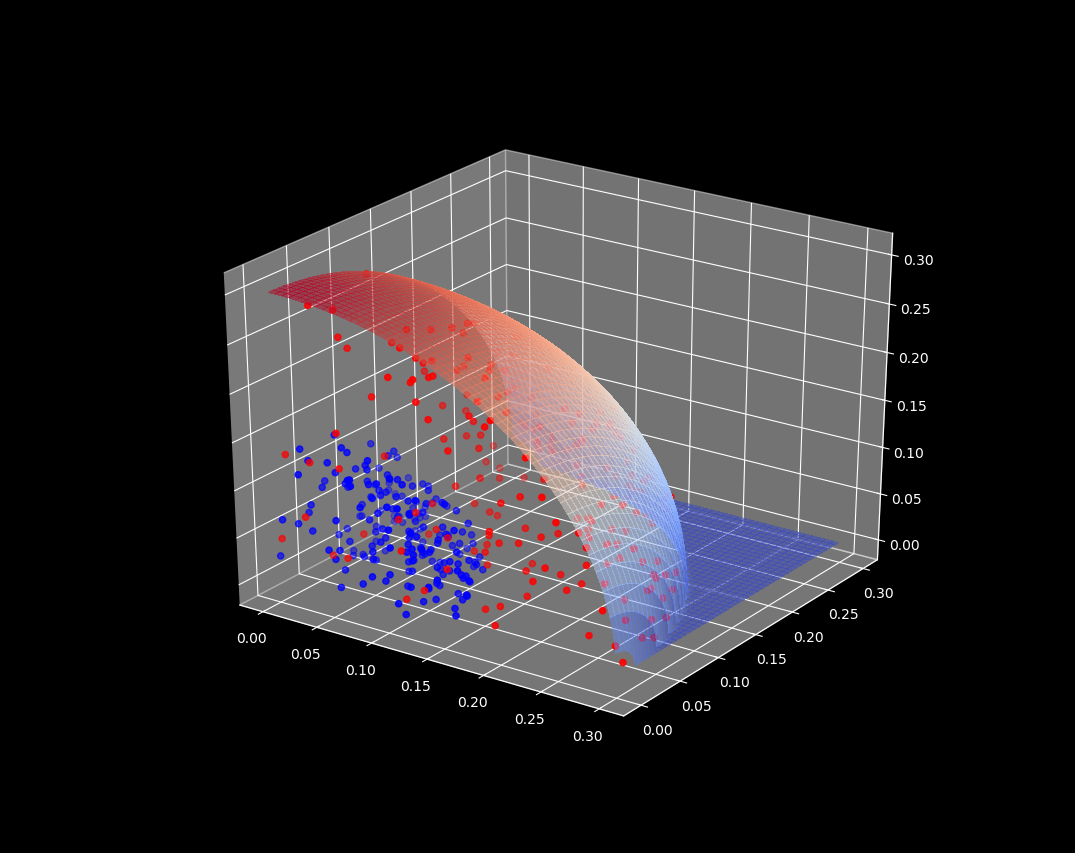
\includegraphics[height=0.9\textheight,trim={0 0 0cm 0},clip]{slide/img_cinematica_inversa/spazio_raggiungibilita.png}
\end{column}
\end{columns}

\note{
Testo validità dei due approcci. Due problemi. 

\# 1 $\to$ problema cinematico inverso puro.

\# 2 $\to$ problema cinematico inverso che cerca di imporre una data forma al manipolatore
}
\end{frame}










\begin{frame}{Ottimizzazione}

    \begin{itemize}
        \item<1->[] Definiamo $\mathrm{directkin}(\vec{\theta})$ la funzione di cinematica diretta del manipolatore.
        \item<2->[] Definiamo $\mathrm{d}(p_1, p_2)$ la distanza tra due punti, $\mathrm{d}_\text{man}(p, \vec{\theta})$ la distanza di un punto $p$ dal manipolatore nella configurazione $\vec{\theta}$.
        \item<3->[] \[ \text{problema1}(\textcolor{red}{\bullet}) = \argmin\limits_{\vec{\theta}} d(\textcolor{red}{\bullet}, \mathrm{directkin}(\vec{\theta})) \]
        sotto i vincoli $|\theta_i| \le \theta_\text{max}$
        \item<4->[] \[ \text{problema2}(\textcolor{red}{\bullet}, \textcolor{blue}{\bullet}) = \argmin\limits_{\vec{\theta}} \Bigg( \alpha \mathrm{d}(\textcolor{red}{\bullet}, \mathrm{directkin}(\vec{\theta})) + (1-\alpha) \mathrm{d}_\text{man}(\textcolor{blue}{\bullet}, \vec{\theta}) \Bigg)\]
        sotto i vincoli $|\theta_i| \le \theta_\text{max}$
    \end{itemize}
    
\note{

    Problema in formule.
    
    1) funzione cinematica del manipolatore
    
    2) funzione dist tra due punti
    
    3) funzione dist tra punto e manipolatore = min distanza del punto da ogni segmento

    \# 1 problema $\to$ funzione costo minimizza distanza tale punto dall'EF. 
    
    \# 2 problema $\to$ funzione costo combinazione lineare della distanza di \# 1 e distanza manipolatore-punto intermedio. $0.5 < \alpha < 1$ poichè posizione end-effector è più importante. 
}

\end{frame}

\begin{frame}{Valutazione degli algoritmi}
\begin{itemize}
\item<1-> quale algoritmo è il migliore?
    \begin{itemize}
        \item<2-> efficiente \Interval
        \item<3-> efficace 
\includegraphics[width=10px]{slide/img_cinematica_inversa/hundred_point_emoji.png}
    \end{itemize}
\end{itemize}
\note{
Efficienza $\to$ quanto tempo impiego a trovare la soluzione

Efficacia $\to$ la percentuale di punti dei quali trovo soluzione
}
\end{frame}

\begin{frame}{Valutazione degli algoritmi: tempi}
\begin{columns}
\begin{column}{0.3\textwidth}
Tempi medi di risoluzione del \emph{Problema 1} su un campione di 200 punti uniformemente distribuiti nello spazio raggiungibile.
\end{column}
\begin{column}{0.7\textwidth}
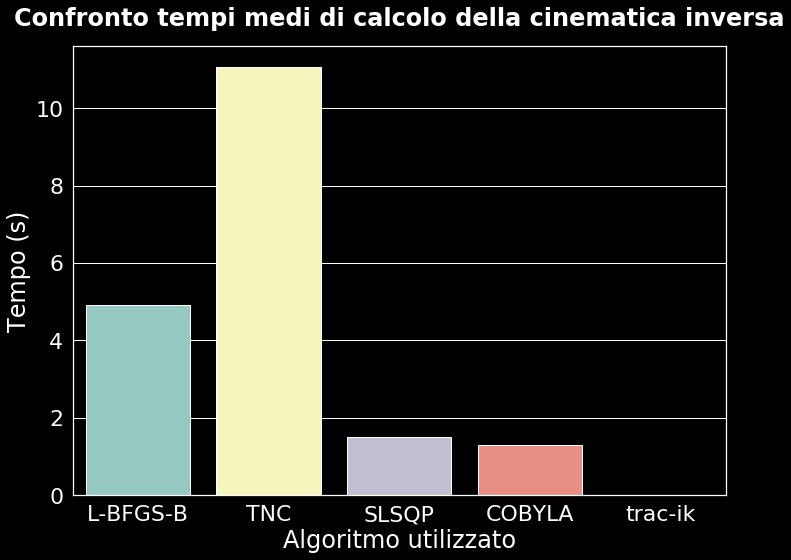
\includegraphics[width=\textwidth]{slide/img_cinematica_inversa/risultati_tempi.png}
\end{column}
\end{columns}

\note{
I tempi medi migliori si hanno sugli algoritmi SLSQP e COBYLA. Gli altri scartati. 

TRAC-IK ha timeout.
}
\end{frame}

\begin{frame}{Valutazione degli algoritmi: errore sulla posizione}
\begin{columns}
\begin{column}{0.3\textwidth}
Errore percentuale sulle soluzioni del \emph{Problema 1} su un campione di 200 punti uniformemente distribuiti nello spazio raggiungibile.
\end{column}
\begin{column}{0.7\textwidth}
\hspace*{-2em}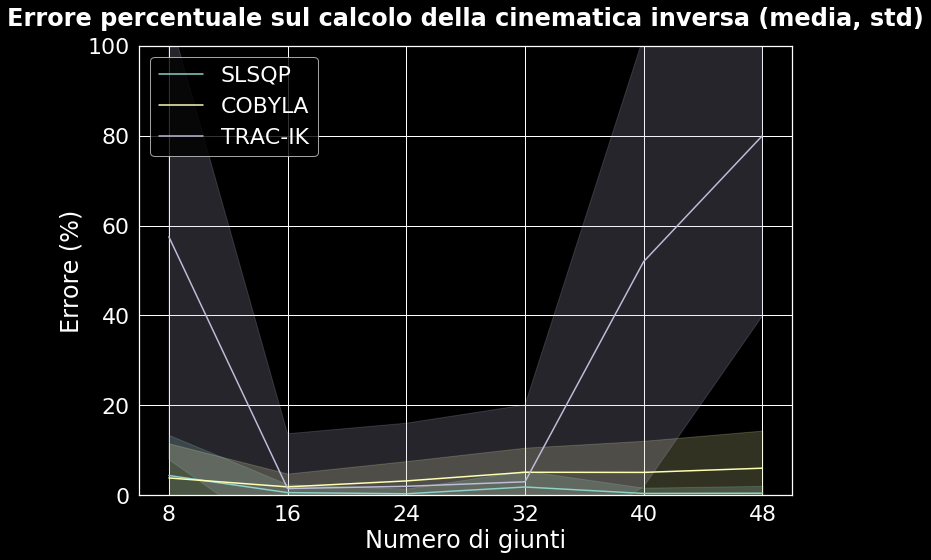
\includegraphics[width=1.15\textwidth]{slide/img_cinematica_inversa/risultati_errore.png}
\end{column}
\end{columns}

\note{
Errore SCIPY costante con i due algoritmi considerati. Errore maggiore con 8GDL.

TRAC-IK molto bene con >16, <32 e molto male altrove. 
}

\end{frame}

\begin{frame}{Valutazione degli algoritmi: accuratezza punti}
\begin{columns}
\begin{column}{0.35\textwidth}
\end{column}
\begin{column}{0.7\textwidth}
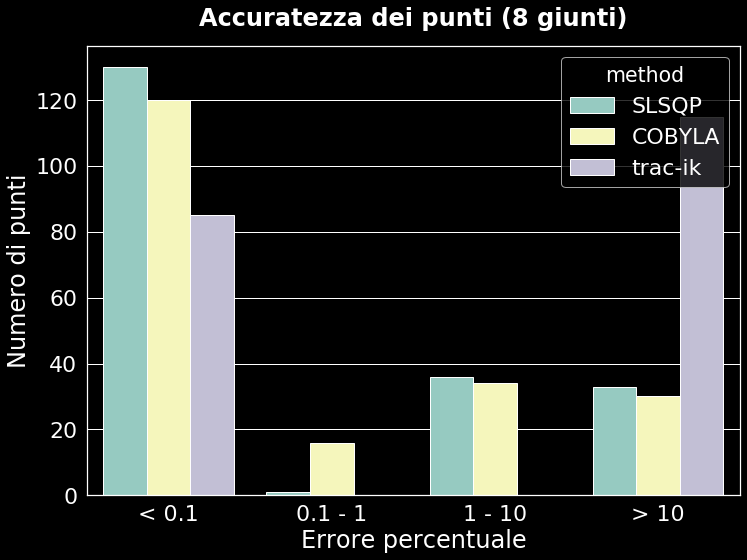
\includegraphics[width=\textwidth]{slide/img_cinematica_inversa/accuratezza_8.png}
\end{column}
\end{columns}

\note{
Accuratezza: 8gdl così così SCIPY (1\%-10\%), male TRAC-IK. 
}
\end{frame}

\begin{frame}{Valutazione degli algoritmi: accuratezza punti}
\begin{columns}
\begin{column}{0.35\textwidth}
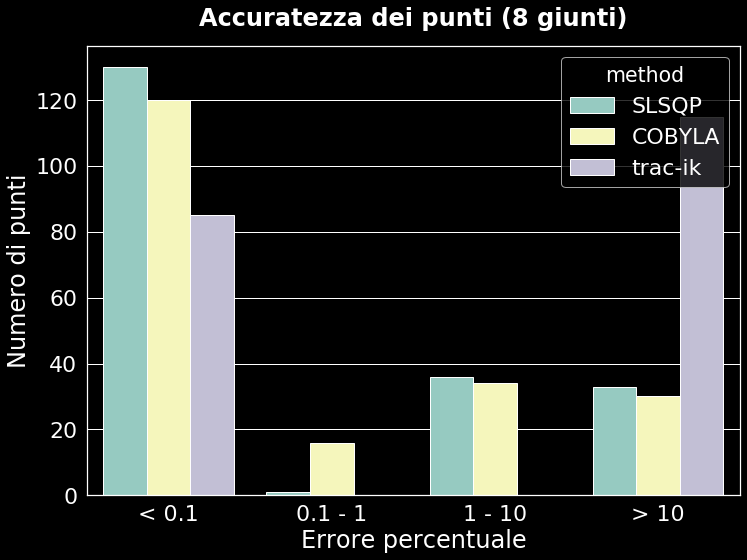
\includegraphics[width=\textwidth]{slide/img_cinematica_inversa/accuratezza_8.png}

\hfill

\end{column}
\begin{column}{0.7\textwidth}
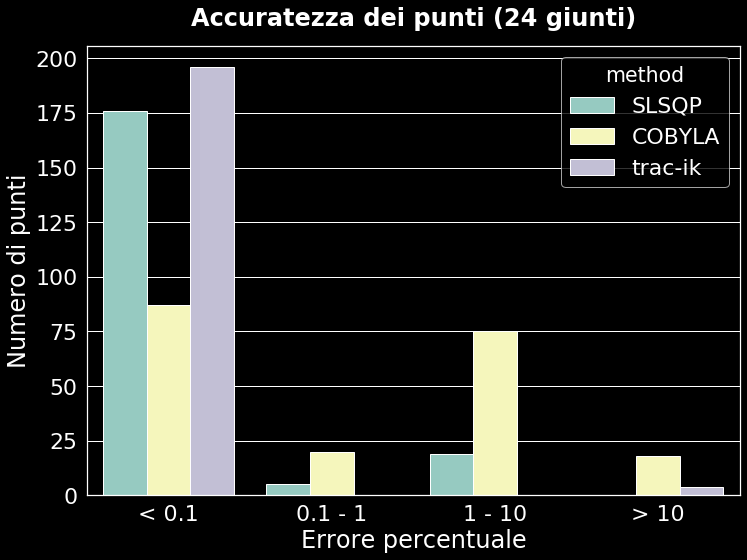
\includegraphics[width=\textwidth]{slide/img_cinematica_inversa/accuratezza_24.png}
\end{column}
\end{columns}

\note{
24 gdl TRAC-IK benissimo. 
}
\end{frame}

\begin{frame}{Valutazione degli algoritmi: accuratezza punti}
\begin{columns}
\begin{column}{0.35\textwidth}
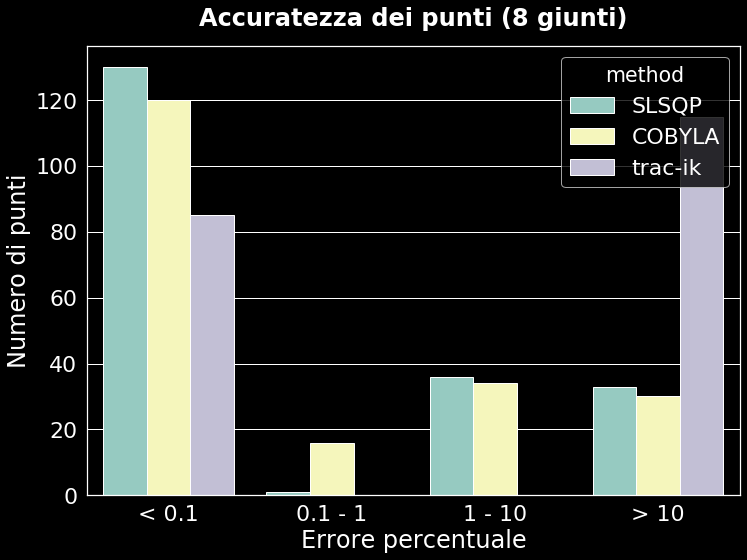
\includegraphics[width=\textwidth]{slide/img_cinematica_inversa/accuratezza_8.png} 

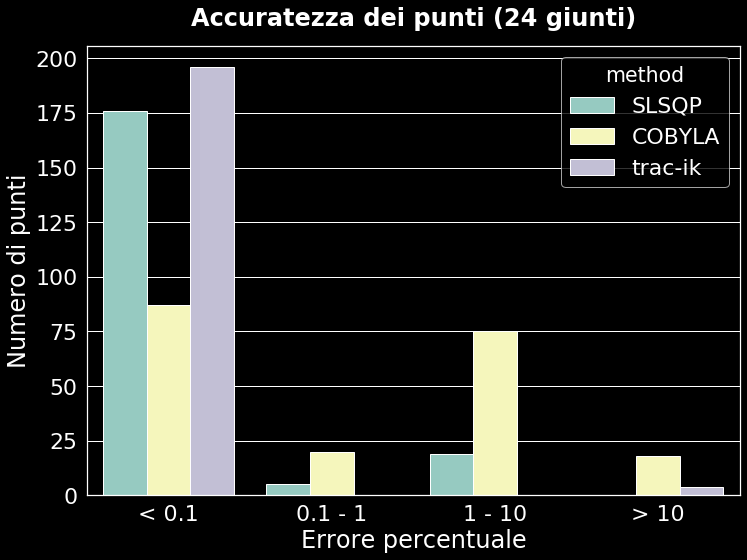
\includegraphics[width=\textwidth]{slide/img_cinematica_inversa/accuratezza_24.png}

\hfill
\end{column}
\begin{column}{0.7\textwidth}
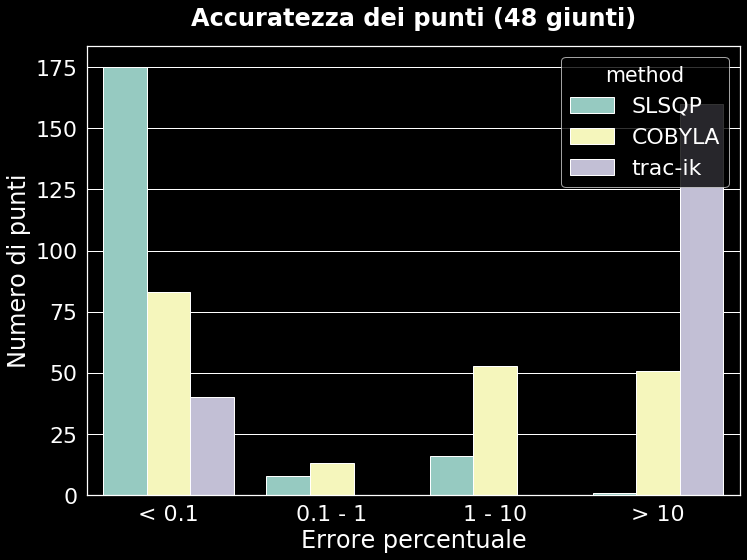
\includegraphics[width=\textwidth]{slide/img_cinematica_inversa/accuratezza_48.png}
\end{column}
\end{columns}
\note{
48 gdl TRAC-IK malissimo. 
}
\end{frame}

\begin{frame}{Valutazione degli algoritmi: \emph{Problema 2}}
\begin{columns}
\begin{column}{0.55\textwidth}
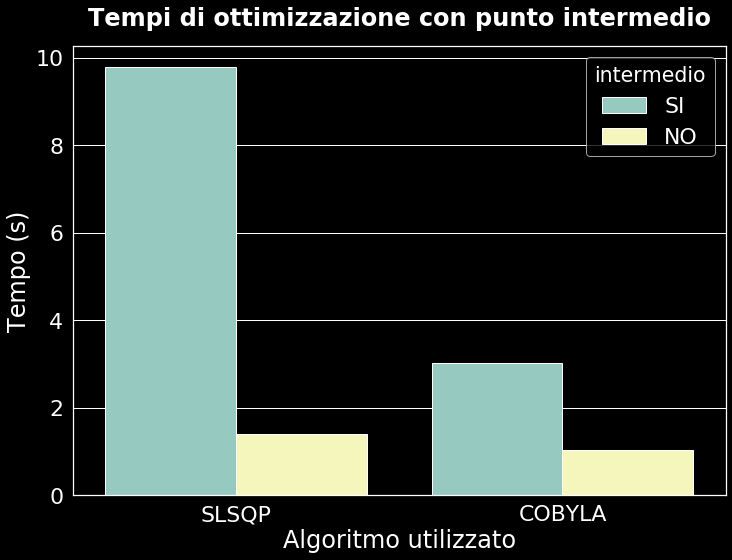
\includegraphics[width=\textwidth]{slide/img_cinematica_inversa/intermedio_tempi.png} 
\end{column}
\begin{column}{0.55\textwidth}
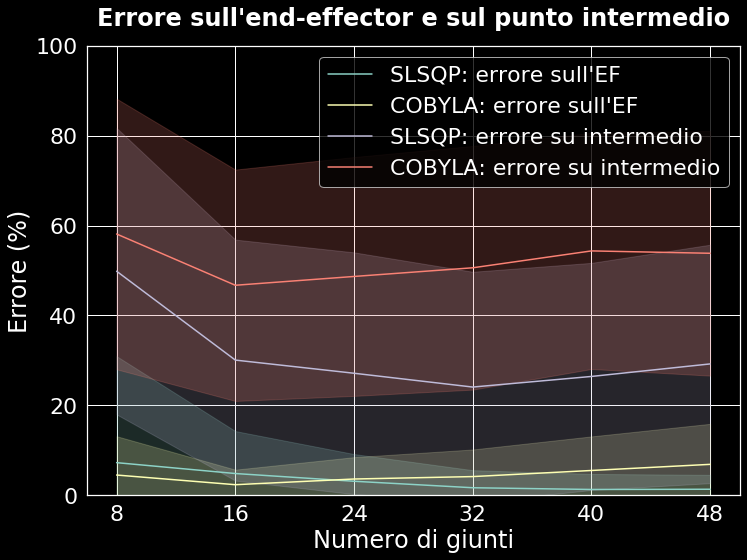
\includegraphics[width=\textwidth]{slide/img_cinematica_inversa/intermedio_errore.png}
\end{column}
\end{columns}
\note{
Non posso confrontare con TRAC-IK poichè non considera punti intermedi. 

Performance temporali SLSQP x5, COBYLA x2. Errore end effector aumenta. Errore punto intermedio alta: posso davvero raggiungere tale il punto principale passando da quello intermedio? Sono generati a caso...
}
\end{frame}

\begin{frame}{Risultati}
\begin{itemize}
\item<1-> TRAC-IK: ottimo con manipolatori di 16-32 giunti 
\includegraphics[width=10px]{slide/img_cinematica_inversa/hundred_point_emoji.png}
\item<2-> SCIPY + SLSQP valida alternativa a TRAC-IK con più di 32 giunti
\begin{itemize}
    \item[\leftthumbsup] posso dare forma al manipolatore
    \item[\leftthumbsdown]<3-> tempi piuttosto lunghi
\end{itemize}
\end{itemize}

\note{
L'approccio proposto da TRAC-IK è ottimo per un numero di giunti compreso tra 16 e 32, sia per i tempi che per l'errore.

Con più di 32 giunti l'approccio migliore è l'algoritmo SLSQP di SCIPY che permette anche di dare forma al manipolatore.

I tempi sono piuttosto lunghi, introdurre un timeout.
}
\end{frame}